\subsection{Settings}
\begin{figure*}[bt]
  \subfigure[Error Ratio\label{fig:er_onestep}]{
  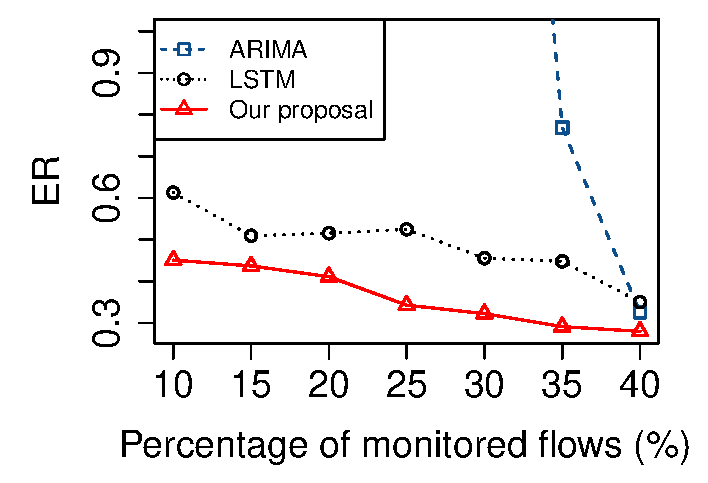
\includegraphics[width=.28\textwidth]{evaluation_figs/ER_one_step_prediciton.eps}
  }
  \subfigure[Root Mean Square Error\label{fig:rmse_onestep}]{
  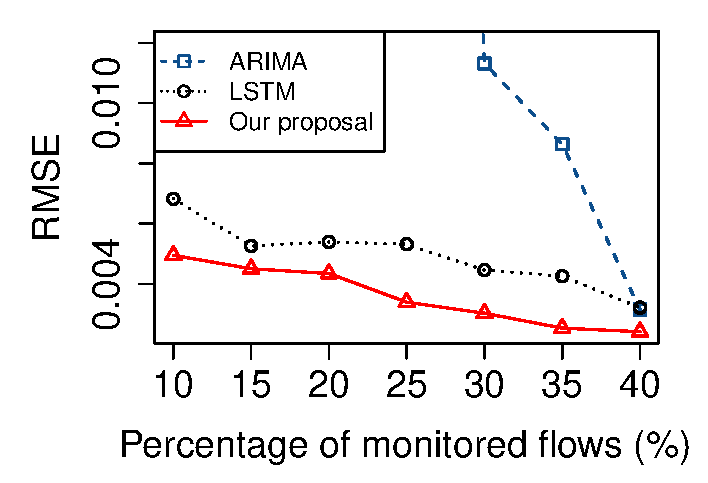
\includegraphics[width=.28\textwidth]{evaluation_figs/RMSE_one_step_prediciton.eps}
  }
  \subfigure[Coefficient of Determination\label{fig:r2_onestep}]{
  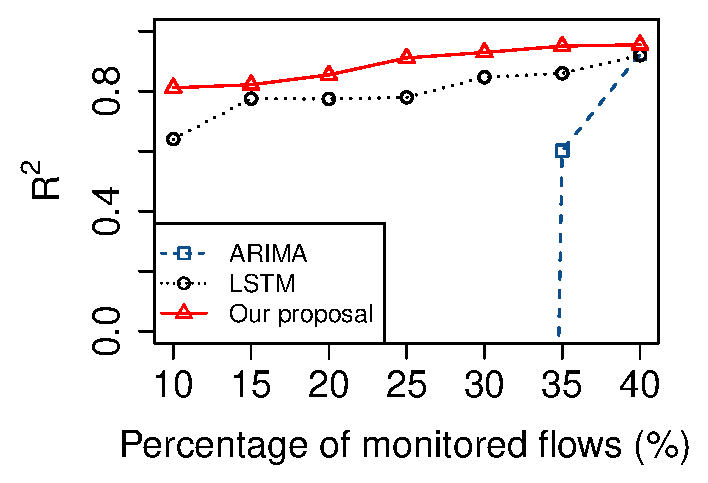
\includegraphics[width=.28\textwidth]{evaluation_figs/R2_one_step_prediciton.eps}
  }
  \vspace{-10pt}
\caption{Performance comparison in one-step-ahead prediction.}
\label{fig:result_onestep_prediction}
\end{figure*}
\begin{figure*}[bt]
  \subfigure[Error Ratio\label{fig:er_multistep}]{
  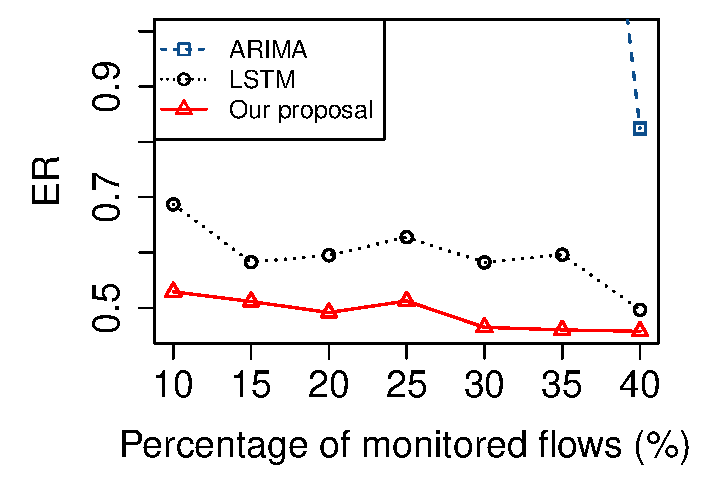
\includegraphics[width=.28\textwidth]{evaluation_figs/ER_multistep_prediciton.eps}
  }
  \subfigure[Root Mean Square Error\label{fig:rmse_multistep}]{
  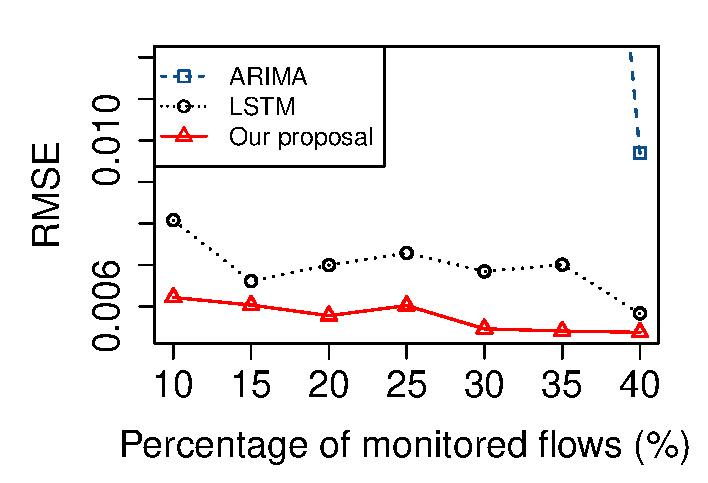
\includegraphics[width=.28\textwidth]{evaluation_figs/RMSE_multistep_prediciton.eps}
  }
  \subfigure[Coefficient of Determination\label{fig:r2_multistep}]{
  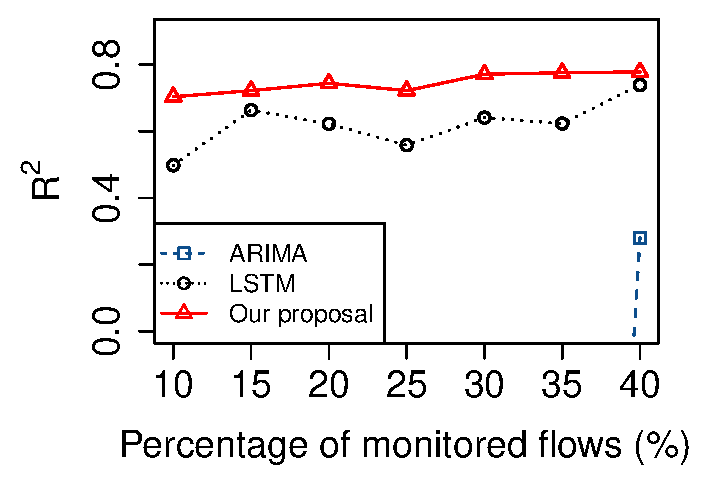
\includegraphics[width=.28\textwidth]{evaluation_figs/R2_multistep_prediciton.eps}
  }
 \vspace{-10pt}
\caption{Performance comparison in multi-step-ahead prediction.}
\label{fig:result_multistep_prediction}
%\vspace{-10pt}
\end{figure*}
\begin{table}
\caption{The configurations of ConvLSTM networks.}
\label{table:convlstm_configurations}
\resizebox{\textwidth}{!}{%
\begin{tabular}{|l|c|l|c|}
\hline
\begin{tabular}[c]{@{}l@{}}Convolutional layers\end{tabular} & 2 & Recurrent dropout & 0.2 \\ \hline
No. of filters & 8/layer & $J$ & 26 \\ \hline
Filter size & (3, 3, 2) & $L$ & 12 \\ \hline
Padding & `same' & No. of trained epoches & 50 \\ \hline
\begin{tabular}[c]{@{}l@{}}CNN dropout\end{tabular} & 0.0 & Batch size & 256 \\ \hline
\begin{tabular}[c]{@{}l@{}}$\lambda_1$, \quad $\lambda_2$\end{tabular} & \begin{tabular}[c]{@{}c@{}}2.0, \quad 1.0\end{tabular} & \begin{tabular}[c]{@{}l@{}}$\lambda_3$, \quad $\lambda_4$\end{tabular} & \begin{tabular}[c]{@{}c@{}}5.0, \quad 0.4\end{tabular} \\ \hline
\end{tabular}%
}
\vspace{-10pt}
\end{table}
We evaluated the performance of our proposed approach by conducting extensive experiments on the Abilene dataset (available at \cite{zhang2011abilene}). The dataset contains the real trace data from the backbone network located in North America which contains 12 nodes ($n = 12$). The Abilene dataset, which includes averages over 5 minutes interval of 144 origin-destination flows from March 1 to September 11, 2004, has been widely used for performance evaluation in many traffic matrix interpolation and prediction studies \cite{xie2015sequential}, \cite{xie2016accurate}. In the experiments, we separated the dataset into 60$\%$ for training, 20$\%$ and 20$\%$ for testing and validating, respectively. We compared our proposal with ARIMA \cite{box2015time} and the standard LSTM model. For ARIMA, we use the historical data of one month as the input for predict future traffic at each timestep. The performance metrics used including Error Ratio ($ER$), Root Mean Square Error ($RMSE$) and Coefficient of Determination (denoted as $R^2$ score) which are defined in (\ref{equation:metrics}). The $ER$ and $RMSE$ are used for measuring the prediction error and the standard deviation of the differences between predicted values and ground-truth values, respectively (the lower values is better). The $R^2$ score determines how well the predicted values are generated by the model. The maximum value of $R^2$ is 1 and it can be a negative number. Moreover, a higher $R^2$ is better.  
\begin{equation}
\label{equation:metrics}
\begin{aligned}
&ER = \frac{\sqrt{\sum_{s,d \in \mathcal{N}}\sum_{i=1}^T{(1-m^i_{s,d})\times(o_{s,d}^i - x_{s,d}^i)^2}}}{\sqrt{\sum_{s,d \in \mathcal{N}}\sum_{i=1}^T{(1-m^i_{s,d})\times(o^i_{s,d})^2}}} \\
&RMSE=\sqrt{\frac{1}{D}\sum_{s,d \in \mathcal{N}}\sum_{i=1}^T{(o^i_{s,d} - x^i_{s,d})^2}}\\
&R^2=1-\frac{\sum_{s,d \in \mathcal{N}}\sum_{i=1}^{T}{(o^i_{s,d}-x_{s,d}^i)^2}}{\sum_{s,d \in \mathcal{N}}\sum_{i=1}^{T}{(o^i_{s,d}-\overline{o}_{s,d}^i)^2}}
\end{aligned}
\end{equation}
where $T$ is the number of timesteps, $D = T \times n \times n$ is the size and $\overline{o}_{s,d}^i = \frac{1}{D}\sum_{s,d \in \mathcal{N}}\sum_{i=1}^{T}{o^i_{s,d}}$ is the mean of the testing dataset. 
The experiments have been conducted on a computer which has Intel i7-6900K CPU @ 3.20GHz, 48 GB memory and two NVIDIA GeForce GTX 1080Ti. The detail configurations of the ConvLSTM networks (the forward and backward networks have the same configurations) are listed in Table \ref{table:convlstm_configurations}.

We conducted two experiments. First, we evaluated the performance of all the three algorithms in one-step-ahead traffic matrix prediction ($L=1$). In the second experiment, we conducted a multi-step-ahead traffic matrix forecasting by predicting the traffic matrices of one hour ahead of the current timestep ($L = 12$). We denote $p$ as the percentage of the monitored flows per timestep. In each experiment, we conducted different scenarios in which $p$ is varied from $10\%$ to $40\%$ (i.e., the maximum number of monitored flows per timestep is $k = p \times n \times n$). 

In the following, we will show the numerical results.
Note that since the values regarding ARIMA are extremely large and lie outside the boundaries of the figures, they are also presented in Table \ref{table:arima_results}. 
%Besides that, we use Table \ref{table:arima_results} to present the results of ARIMA approach in both one-step-ahead prediction (i.e., the left value) and multi-step-ahead prediction (i.e., the right value) since the values are extremely large and lie outside the boundaries of the figures. 
\subsection{One-step-ahead traffic prediction results}
%we made the traffic prediction with different values of $k$ ($k$ is the number of monitored flows in each timestep). $k$ is equal to 10$\%$, 15$\%$, 20$\%$,...,40$\%$ of the total number of flows (i.e., $n \times n$).
In this section, we present the performance evaluation in one-step-ahead traffic prediction.
First, we evaluate how well the algorithms can capture the traffic trend (Fig.\ref{fig:prediction_result}). 
%by first show the comparison of the overall performance of all algorithm in Fig.\ref{fig:prediction_result}. 
The figure shows the difference between the predicted values and the actual values of a flow chosen randomly in about 6 hours (with 30$\%$ flows are monitored). As shown, our algorithm can capture the traffic trend much more smoothly compared with the other two algorithms. 
Besides that, thanks to the monitoring policy (described in Section \ref{subsection:flows_selection}), our proposal monitors the traffic at more spikes than ARIMA and LSTM (which use simple random policies in deciding monitored flows). 
%our proposal performs better in determining the time to monitor the flow at the spike, compared with the random policy used in ARIMA and LSTM approaches. 

Fig.\ref{fig:result_onestep_prediction} shows the performance comparison among ARIMA, LSTM and our proposed approach in terms of the Error Ratio, Root Mean Square Error and Coefficient of Determination. 
%In overall, the LSTM and ConvLSTM approaches show the superiority in modeling and predicting the temporal sequence when their results outperform the ARIMA approach in terms of all metrics. 
It can be seen that our proposal achieves the best performance regarding all the metrics. LSTM shows the second best performance and ARIMA is the worst. Comparing LSTM and our proposal, we can see that our approach achieves a high accuracy in most of the experiment scenarios. Specifically, in the best case (i.e., $p=35\%$ flows are monitored), the $ER$ and $RMSE$ of our algorithm are 35.0$\%$ and 40.5$\%$ less than that of LSTM, respectively. 
In terms of $R^2$ score, our proposal achieves 26.7$\%$ better than the LSTM approach in the best case (i.e., $p=10\%$). Moreover, it can be seen that our proposal in case $p=25\%$, achieves better performance (regarding all metrics) as LSTM in case $p=40\%$.
%our approach shows the same performance (in all metrics) while requires only 25$\%$ of ground-truth input comparing with 40$\%$ in case of using LSTM.
%(i.e., the ratio of monitored flows). 
 %Specifically, in the case of using 35$\%$ ground-truth data as input, our proposed approach results in the $ER$ and $RMSE$ that are less than 39.8$\%$ and 44.9$\%$ that of LSTM, respectively. In term of $R^2$ score, we achieve 12$\%$ better than LSTM approach.
%In addition, Fig.\ref{fig:result_onestep_prediction} indicates that while the results of our approach steadily decreases (in terms of $ER$ and $RMSE$) or increases (in terms of $R^2$ score) when increasing the ratio of the monitored flows, LSTM does not. 
%the figures of LSTM shows the dynamic in the trend. 
In addition, Fig.\ref{fig:result_onestep_prediction} indicates that while the performance of our proposal is improved gradually when increasing the number of monitored flows, LSTM does not.
The fluctuation in the results of LSTM can be explained by the random policy in choosing flows to be monitored after each timestep. 

The ratio of ground-truth input has a massive impact on the prediction accuracy of ARIMA. As shown in Table \ref{table:arima_results}, when $p < 25\%$, we see the dramatical increase of $ER$ and $RMSE$. Specifically, when $p = 10\%$, $ER$ and $RMSE$ become extremely large, i.e., $ER=2.45\mathrm{e}10$, $RMSE=3.27\mathrm{e}8$.
%from 7.27 to 2.45e10 and from 0.07 to 3.27e8 in $ER$ and $RMSE$, respectively. 
Similarly, the $R^2$ score also makes a huge decrease from $-41.23$ to $-5.27\mathrm{e}20$ when reducing $p$ from $25\%$ to $10\%$. However, when the percentage of ground-truth data in the input is sufficiently large (i.e., $p = 40\%$), ARIMA can performs very well and its performance is close to that of our algorithm. This results strongly emphasizes the advantage of our model in predicting the future traffic with only a small portion of ground-truth information.

% Please add the following required packages to your document preamble:
% \usepackage{graphicx}
\begin{table}[]
\caption{The prediction results of ARIMA}
\label{table:arima_results}
\resizebox{\textwidth}{!}{%
\begin{tabular}{|c|c|c|c|}
\hline
\begin{tabular}[c]{@{}l@{}}$p$\end{tabular} & $ER$ (exp1$|$exp2) & $RMSE$ (exp1$|$exp2)& $R^2$ (exp1$|$exp2)\\ \hline
$10\%$ & $2.45\mathrm{e}10$ $|$ $7.29\mathrm{e}10$ & $3.27\mathrm{e}8$ $|$ $1.05\mathrm{e}9$ & $-5.72\mathrm{e}20$ $|$ $-5.8\mathrm{e}21$ \\ \hline
$15\%$ & $3.5\mathrm{e}6$ $|$ $1.001\mathrm{e}7$ & $4.5\mathrm{e}4$ $|$ $1.4\mathrm{e}5$ & $-1.1\mathrm{e}13$ $|$ $-1.09\mathrm{e}14$\\ \hline
$20\%$ & $40220$ $|$ $158861$ & $323.75$ $|$ $1406$ & $-1.48\mathrm{e}9$ $|$ $-2.8\mathrm{e}10$\\ \hline
$25\%$ & $7.27$ $|$ $17.98$ & $0.07$ $|$ $0.21$ & $-41.23$ $|$ $-341.6$\\ \hline
$30\%$ & $2.89$ $|$ $11.5$ & $0.032$ $|$ $0.087$ & $-13.6$ $|$ $-148.2$ \\\hline
$35\%$ & $0.77$ $|$ $2.04$ & $0.008$ $|$ $0.03$ & $0.62$ $|$ $-3.58$ \\ \hline
$40\%$ & $0.33$ $|$ $0.83$ & $0.003$ $|$ $0.009$ & $0.92$ $|$ $0.28$\\ \hline
\end{tabular}%
}
\vspace{-10pt}
\end{table}
\subsection{Multi-step-ahead traffic prediction results}
In this section, we present the results of multi-step-ahead traffic prediction under various settings of the ratio of the monitored flows. 
In each timestep, our proposed algorithm and LSTM predict the traffic matrices of one hour ahead by applying the IMS approach, while ARIMA uses the Direct Multi-Step approach.
%In each timestep, we forecast the traffic matrices of one hour ahead by applying the IMS approach (except that ARIMA uses the Direct Multi-Step approach). 

Fig.\ref{fig:result_multistep_prediction} shows the performance evaluation of all the three algorithms in terms of $ER$, $RMSE$ and $R^2$ score.
In general, similar to the first experiment, our approach achieves the best performance in all scenarios, followed by LSTM and ARIMA. In comparison with LSTM, 
in the best case (i.e., 10$\%$ of flows are monitored), the  $ER$, $RMSE$ of our algorithm are about 23.0$\%$ less than that of LSTM. 
Moreover, our algorithm results in the $R^2$ score that is 41.2$\%$ less than LSTM.  
%our proposal decreases 0.167 (24.6$\%$), 0.00197 (24.62$\%$), and improves 0.211 (29.4$\%$) in terms of $ER$, $RMSE$, and $R^2$ score, respectively. 
Similar to the first experiment, ARIMA also shows very poor performance compared to the other two approaches. 

Comparing the results of the two experiments, it can be seen that the performance of the three algorithms in the second experiment is worse than that in the first experiment. 
However, the degradation of ARIMA is much more larger than that of our approach and LSTM. 
Specifically, in the best case (i.e., the percentage of the monitored flows is 10$\%$), the prediction errors of our approach and LSTM increase by only 17.3$\%$ and 12.5$\%$, respectively, while that of ARIMA is 197.6$\%$. 
%Considering the performance of the three algorithms in the two experiments, it can bee seen that the per
%Comparing the performance of the algorithms 
%We make the comparison between the results of the second experiment with the previous one. 
%Considering the best case, the prediction error of our approach and LSTM only increase 17.02 $\%$ and 11.14$\%$, respectively, while this value of ARIMA is 147.3$\%$. In addition, the increasings in term of $RMSE$ are 25$\%$, 18$\%$, and 184$\%$. In $R^2$ score, despite of achieving a high value (in case $p = 40\%$) in the on-step-ahead prediction, this value of ARIMA drops 70$\%$ in the second experiment. This drop of our model and LSTM are $18.5\%$ and $19.27\%$ respectively.

In summary, by applying the Convolutional LSTM network and the forward/backward data correction technique, our proposal shows the superiority in handling the missing ground-truth in the historical data.
Specifically, our proposed algorithm reduces the $ER$, $RMSE$ and increases the $R^2$ significantly compared to LSTM and ARIMA. 
%in order to achieve the high accurate traffic matrix prediction in both experiments.

% It can be seen that the performance of all algorithms in multi-step-ahead prediction is worse than that in one-step-ahead prediction. Moreover, the gap between the performance of the two experiments of our proposal and LSTM is greater than that of ARIMA. This can be explained by the use of IMS.
% %However, due to applying the IMS for multi-step prediction, the LSTM and our approach are witnessed a considerable loss in the performance evaluation in terms of all metrics. 
% For example, regarding the $ER$, while ARIMA only increases the error by y$\%$, those values of LSTM and our proposal are increased by 10$\%$ and 14.6$\%$, respectively. 
% %LSTM and our algorithm suffer the high loss in the second experiment since they use the IMS approach while the ARIMA use the Direct Multi-Step (DMS) approach for predicting multi traffic matrices. 
% Indeed, the authors in \cite{shi2018machine} have proved that DMS is more accurate than the IMS but it is difficult to train.
% \begin{table}[]
% \resizebox{\textwidth}{!}{%
% \caption{The configurations of ConvLSTM networks.}
% \label{table:convlstm_configurations}
% \begin{tabular}{|l|c|l|c|}
% \hline
% \multicolumn{4}{|c|}{ConvLSTM configurations}                                                                                                                                                    \\ \hline
% \begin{tabular}[c]{@{}l@{}}Number of \\ Convolutional \\ layer\end{tabular} & 2                        & Recurrent Dropout                                                                    & 0.0 \\ \hline
% Number of fillers                                                        & 8/layer                  & \begin{tabular}[c]{@{}l@{}}$J$ (No. of previous\\  traffic matrices)\end{tabular}      & 26  \\ \hline
% Kernel size                                                                   & (3, 3)                   & \begin{tabular}[c]{@{}l@{}}$L$ (No. of timesteps \\ in multi-step \\ prediction)\end{tabular} & 12  \\ \hline
% Padding                                                                  & 'same'                   & Training epochs                                                                      & 50  \\ \hline
% \begin{tabular}[c]{@{}l@{}}Convolutional \\ Dropout\end{tabular}                                                                  & \multicolumn{1}{c|}{0.2} & Batch size                                                                           & 256 \\ \hline
% \begin{tabular}[c]{@{}l@{}}$\lambda_1$ \\ $\lambda_2$\end{tabular}                                                                  & \multicolumn{1}{c|}{2\\1} & $\lambda_3$\\$\lambda_4$                                                                           & {5\\0.4} \\ \hline
% \end{tabular}%
% }
% \end{table}